\documentclass{article}
\usepackage{graphicx}
\usepackage{booktabs}
\usepackage{hyperref}
\title{Agentic Reliability Framework v1.0.4}
\author{Agentic Reliability Framework Contributors}
\date{2025}
\begin{document}
\maketitle
% Auto-generated by scripts/write_spec_hash.sh
\newcommand{\ARFSpecVersion}{1.0.4}
\newcommand{\ARFSpecHash}{sha256:126e444de22141ea1f24b53949a277fd12b0eb3f25df4a097541e81516b793a3}
\newcommand{\ARFSpecFiles}{\detokenize{spec/ACJ_PROTOCOL_v1_0_4.md,spec/ARF_NORMATIVE_REQUIREMENTS_INDEX_v1_0_4.md,spec/ARF_PATCH_LEDGER_v1_0_4.md,spec/ARF_RUNTIME_CONTRACT_v1_0_4.md,spec/ARF_STATE_VECTOR.schema.v1_0_4.json}}


\begin{abstract}
The Agentic Reliability Framework (ARF) specifies a minimal runtime contract,
change journal protocol, and patch ledger that together provide auditability
for agentic systems. This paper summarizes the v1.0.4 release and highlights
the interoperability and security requirements.
\end{abstract}

\section{Introduction}
Agentic systems require consistent telemetry, change tracking, and verification
mechanisms to safely evolve. ARF defines three core artifacts: a runtime
contract for event streams, an Agentic Change Journal (ACJ) protocol, and a
patch ledger for applied fixes. These artifacts provide traceability from
runtime observations to remediation.

The compiled paper embeds a deterministic hash of the v\ARFSpecVersion{}
specifications to ensure any spec edits produce a detectable change in the PDF.
Spec hash: \texttt{\ARFSpecHash}.

\section{System Overview}
Figure~\ref{fig:architecture} summarizes how runtime telemetry, ACJ entries, and
patch ledger updates connect to monitoring and governance workflows.

\begin{figure}[h]
  \centering
  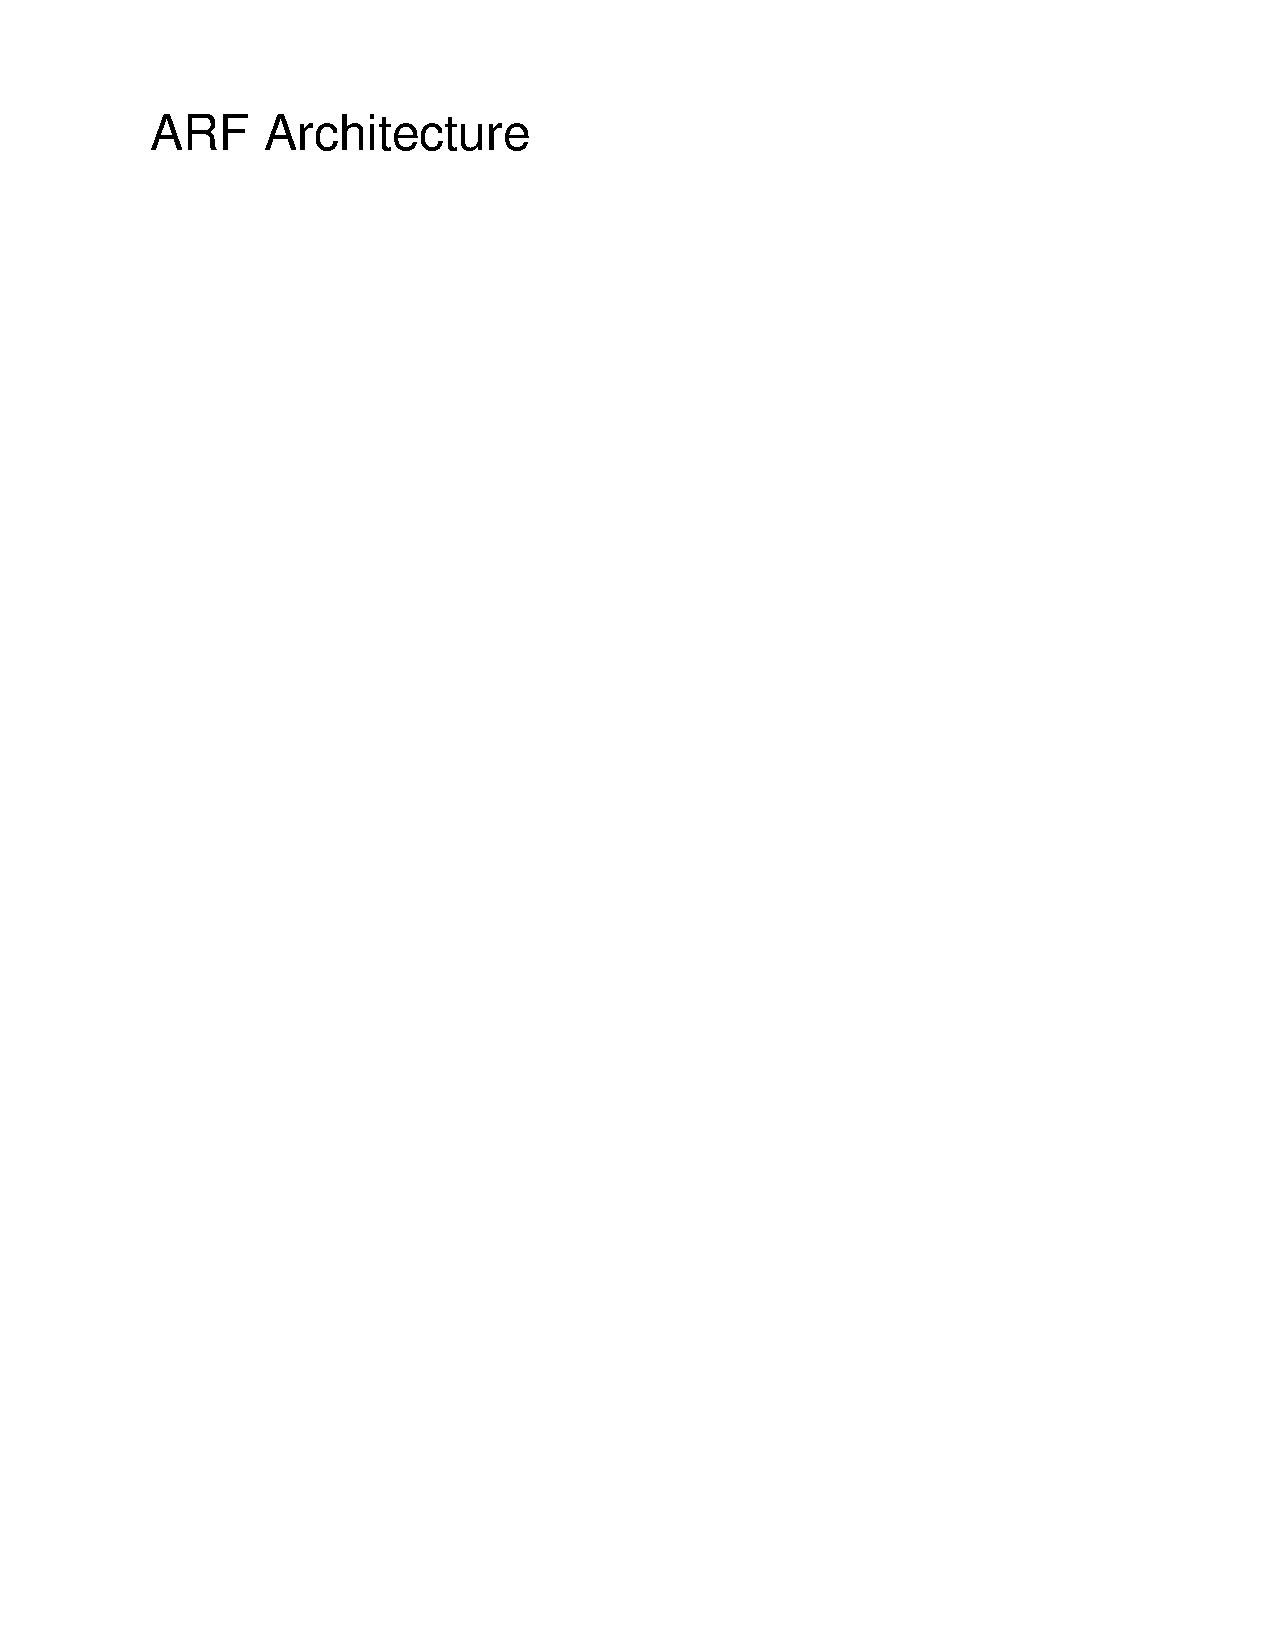
\includegraphics[width=0.9\linewidth]{figures/arf_architecture.pdf}
  \caption{ARF telemetry and change-control flow.}
  \label{fig:architecture}
\end{figure}

\section{Runtime Contract}
The runtime contract specifies task lifecycle events, state vector snapshots,
and remediation records. State vectors must conform to the v1.0.4 schema and
include inputs, outputs, tool usage, confidence, and policy references.

\section{Agentic Change Journal}
ACJ entries record material changes in behavior, configuration, or policy. Each
entry references evidence from runtime telemetry and links to patch ledger
records when changes are applied.

\section{Patch Ledger}
The patch ledger is an append-only log of applied patches, with each record
linking back to the motivating ACJ entry. Integrity metadata is recommended to
ensure auditability across the system lifecycle.

\section{Formal Invariants and Properties}
The ARF release specifies a small set of invariants and properties that must
hold across implementations:
\begin{itemize}
  \item \textbf{I1 (State Vector Completeness)}: every task lifecycle event
  yields a state vector snapshot with required inputs, outputs, tool calls, and
  policy references. \textit{Enforced by}: runtime contract validators and
  schema checks.
  \item \textbf{I2 (Traceability)}: every behavioral change has a corresponding
  ACJ entry that references evidence and, if applicable, a patch ledger record.
  \textit{Enforced by}: ACJ protocol requirements and patch ledger linkage.
  \item \textbf{P1 (Immutable Audit Trail)}: once recorded, ACJ and patch ledger
  entries are append-only and never overwritten. \textit{Enforced by}: ledger
  append-only storage plus integrity metadata.
  \item \textbf{P2 (Policy-Scoped Actions)}: tool calls and outputs are scoped to
  active policy identifiers in the state vector. \textit{Enforced by}: runtime
  contract fields with policy references.
  \item \textbf{P3 (Evidence-Bound Remediation)}: patches must cite evidence from
  runtime telemetry or ACJ records. \textit{Enforced by}: patch ledger evidence
  references and review workflows.
  \item \textbf{P4 (Conformance Gate)}: releases are valid only when schema
  checks, paper build, and arXiv bundle packaging succeed. \textit{Enforced by}:
  CI conformance checks and release scripts.
\end{itemize}

\section{Threat Model}
\begin{table}[h]
  \centering
  \begin{tabular}{p{0.28\linewidth} p{0.42\linewidth} p{0.22\linewidth}}
    \toprule
    Attack & Mitigation & Residual Risk \\
    \midrule
    Tampering with telemetry streams &
    Schema-validated state vectors, integrity metadata, and ACJ evidence
    requirements & Low: requires breaking both telemetry and ledger \\
    Drift between runtime behavior and recorded changes &
    ACJ linkage to evidence and patch ledger references & Medium: requires
    disciplined review workflows \\
    Unauthorized tool invocation &
    Policy-scoped tool call fields and runtime contract validation &
    Medium: depends on policy enforcement rigor \\
    Silent spec changes &
    Embedded spec hash in the paper and versioned spec filenames &
    Low: changes surface in builds \\
    \bottomrule
  \end{tabular}
  \caption{Threat model for ARF deployments.}
\end{table}

\section{Conformance Test Plan}
An implementation is ARF-compliant when the following checks pass:
\begin{enumerate}
  \item \textbf{Schema validation}: generated state vectors validate against
  the v1.0.4 schema for representative task runs.
  \item \textbf{Lifecycle coverage}: task start, tool invocation, output, and
  remediation events are emitted and linked consistently.
  \item \textbf{ACJ integrity}: each behavioral or policy change yields an ACJ
  entry referencing evidence and (if applicable) a patch ledger record.
  \item \textbf{Patch ledger integrity}: patch entries are append-only and point
  back to the triggering ACJ entry.
  \item \textbf{Release checks}: schema sanity, paper build, and arXiv bundle
  packaging complete without errors.
\end{enumerate}

\section{Ablation Analysis}
Removing ARF components produces measurable reliability regressions:
\begin{itemize}
  \item \textbf{Without the monitor}: telemetry gaps eliminate evidence needed
  for ACJ entries, undermining traceability and preventing repeatable audits.
  \item \textbf{Without receipts (ACJ entries)}: behavioral changes lose causal
  linkage, making it impossible to prove when or why updates occurred.
  \item \textbf{Without the tool gateway}: tool usage becomes unscoped, which
  increases the risk of policy violations and complicates post-incident reviews.
\end{itemize}

\section{Conclusion}
ARF v1.0.4 provides a concise, interoperable approach to reliability and
observability for agentic systems. Future work will expand adapter guidance and
formal validation tooling.

\bibliographystyle{plain}
\bibliography{arf}
\end{document}
